\documentclass[xcolor=table,dvipsnames,table]{beamer}
\mode<presentation>
\usetheme{boxes}
\setbeamertemplate{navigation symbols}{}
% http://www.latex-community.org/forum/viewtopic.php?f=4&t=6694
\setbeamertemplate{navigation symbols}{\raisebox{5pt}{\makebox[\paperwidth]{\hfill\makebox[10pt]{\scriptsize\insertframenumber\vspace{1ex}}}}}
%\setbeamertemplate{footline}[frame number]
\setbeamertemplate{blocks}[shadow=false]
%\setbeamercolor*{block title}{fg=structure,bg=RoyalBlue!10}
\setbeamercolor*{block title example}{fg=structure,bg=RoyalBlue!10}
%\setbeamercolor*{block title example}{fg=BrickRed,bg=Goldenrod!10}
\setbeamercolor*{block title alerted}{fg=white,bg=black}
\addtobeamertemplate{block begin}{\pgfsetfillopacity{0.8}}{\pgfsetfillopacity{1}}
%\rowcolors{0}{RoyalBlue!20}{RoyalBlue!5}
\setbeamertemplate{caption}{\raggedright\insertcaption\par}

%\DeclareGraphicsRule{*}{mps}{*}{}

\usepackage{latexsym}
\usepackage{hyperref}
\usepackage{tikz}
\usetikzlibrary{calc,shapes,arrows,shadows,shapes.callouts,shapes.arrows,chains,positioning,trees}
\usepackage{solution}
\usepackage{calc}
\usepackage{pifont}
\usepackage{algorithmic}
\usepackage{pdfcomment}
\usepackage{color}

\newcommand{\cmark}{\ding{51}}
\newcommand{\xmark}{\ding{55}}

\newcommand{\highlight}[1]{{\color{blue}{#1}}}
\newcommand{\mycite}[1]{{\color{darkgray}{\footnotesize [#1]}}}

\DeclareMathOperator*{\argmin}{arg\,min}
\DeclareMathOperator*{\argmax}{arg\,max}
\DeclareMathOperator{\sign}{sign}
\DeclareMathOperator{\cnt}{Count}

\newcounter{mycallout}

\newcommand{\callouts}[3]{%
  \stepcounter{mycallout}
  \tikz[remember picture,baseline]{\node[anchor=base,inner sep=0,outer sep=0]%
    (\themycallout) {\colorbox{#1!20}{#3}};\pause\node[overlay,rectangle callout,%
    callout relative pointer={(0cm,0.5cm)},fill=#1!20] at ($(\themycallout.south)+(-0cm,-0.7cm)$){#2};}%
    }%

\raggedright

\newcount\lecturecount
\lecturecount=0
\AtBeginLecture{%
    \advance\lecturecount by 1
    \date{}
    \begin{frame}
    \begin{center}
    \titlepage
    \ifnum\lecturecount=1
    Part \the\lecturecount: \insertlecture
    \else
    Part \the\lecturecount: \insertlecture
    \fi
    \end{center}
    \end{frame}
}

\addtobeamertemplate{block begin}{\setlength\abovedisplayskip{0pt}}

%\newcommand{\example}[1]{{\color{BrickRed!50}{#1}}}
\newcommand{\maths}[1]{{\color{RoyalBlue!50}{#1}}}
\newcommand{\reference}[1]{{\color{RoyalBlue!30}\tiny [from #1]}}
\newcommand{\koehnref}{\reference{\href{http://www.statmt.org/book}{P.Koehn SMT book slides}}}


\begin{document}

\title{\color{MidnightBlue}Natural Language Processing}

\author{Anoop Sarkar \\ {\color{RoyalBlue!70}{\href{http://anoopsarkar.github.io/nlp-class}{anoopsarkar.github.io/nlp-class}}}}
\institute{\color{BrickRed}Simon Fraser University}
%\date{}
     
{
\addtocounter{framenumber}{-1}
\begin{frame}
\begin{center}
\vspace{8mm}

\includegraphics[scale=0.35]{figures/natlang-cky-logo}
\end{center}
\titlepage
\end{frame}
}



\lecture{Word Vectors}{}

\section{One-hot vectors}
\frame{\tableofcontents[currentsection]}

\begin{frame}
\frametitle{One-hot vectors}
\begin{itemize}[<+->]
\item Let $|V|$ be the size of the vocabulary
\item Assign each word to a unique index from $1 \ldots |V|$
\item e.g. {\em aarvark} is $1$, {\em a} is $2$, etc.
\item Represent each word as as a $\mathbb{R}^{|V|\times 1}$
\item The vector has one at index $i$ and all other values are $0$
\end{itemize}
\end{frame}

\begin{frame}
\frametitle{One-hot vectors}
\framesubtitle{Figure from \cite{cs224n}}
\begin{center}
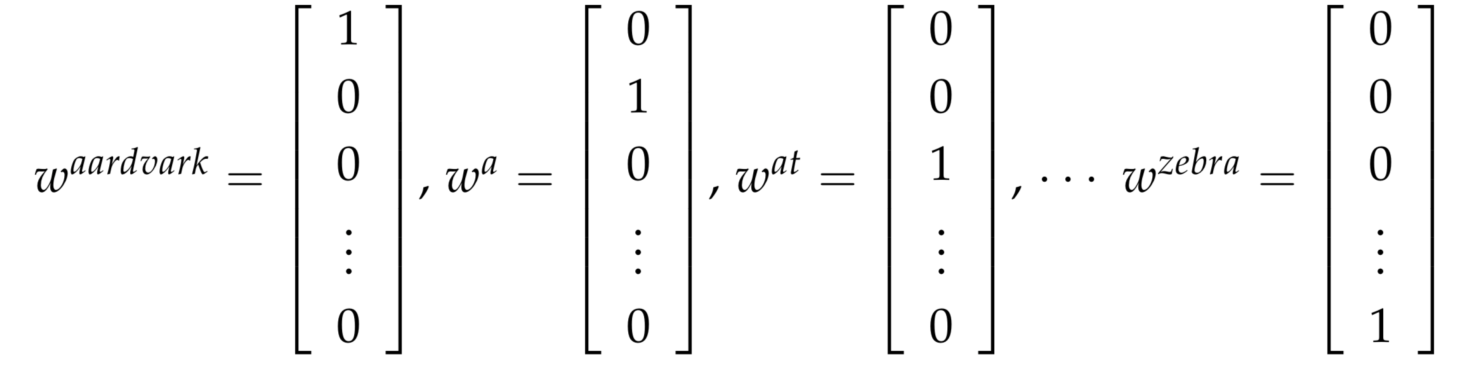
\includegraphics[scale=.45]{figures/wordvectors/onehot}	
\end{center}
\end{frame}

\begin{frame}
\frametitle{One-hot vectors}
\begin{itemize}[<+->]
\item Problems with similarity over one-hot vectors 
\item Consider similarity between words as dot product between their word vectors:
\[ w_{\textrm{cat}} \cdot w_{\textrm{dog}} = 
w_{\textrm{joker}} \cdot w_{\textrm{dog}} = 
0 \]
\item Idea: reduce the size of the large sparse one-hot vector
\item Embed large sparse vector into a dense subspace.
\end{itemize}
\end{frame}

\section{Singular Value Decomposition}
\frame{\tableofcontents[currentsection]}

\begin{frame}
\frametitle{Window based co-occurrence matrix}
\begin{itemize}[<+->]
\item Assume a window around each word (window size 2, 5, $\ldots$)
\item Collect co-occurrence counts for each pair of words in the vocabulary.
\item Create a matrix $X$ where each element $X_{i,j} = c(w_i, w_j)$
\item $c(w_i, w_j)$ is the number of times we observe word $w_i$ and $w_j$ together
\item $X$ is going to be very sparse (lots of zeroes)
\end{itemize}
\end{frame}

\begin{frame}
\frametitle{Window based co-occurrence matrix}
\begin{center}
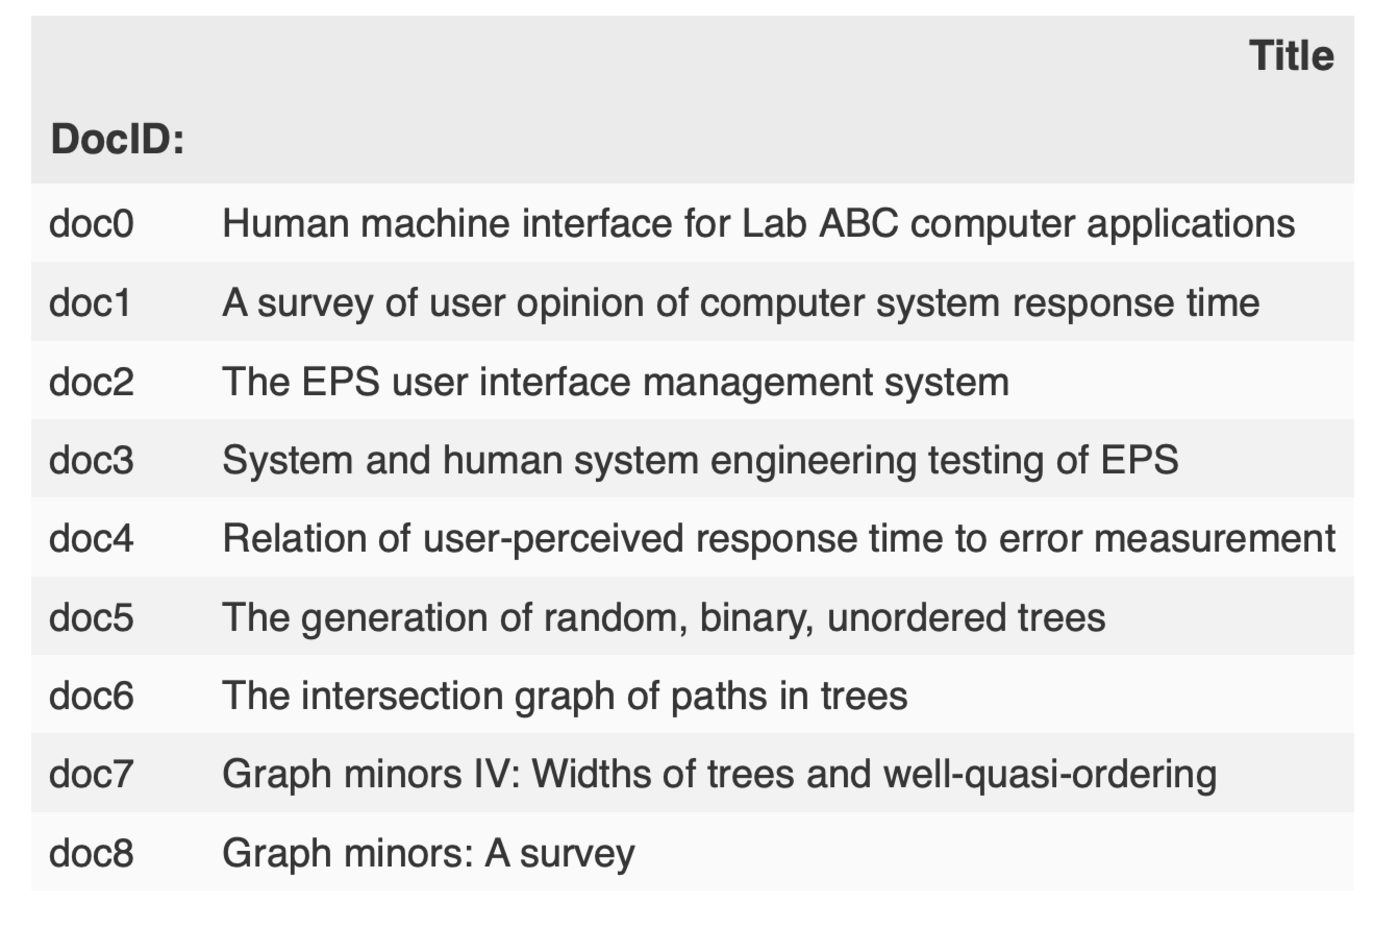
\includegraphics[scale=.45]{figures/wordvectors/docs}	
\end{center}
\end{frame}

\begin{frame}
\frametitle{Window based co-occurrence matrix}
\begin{center}
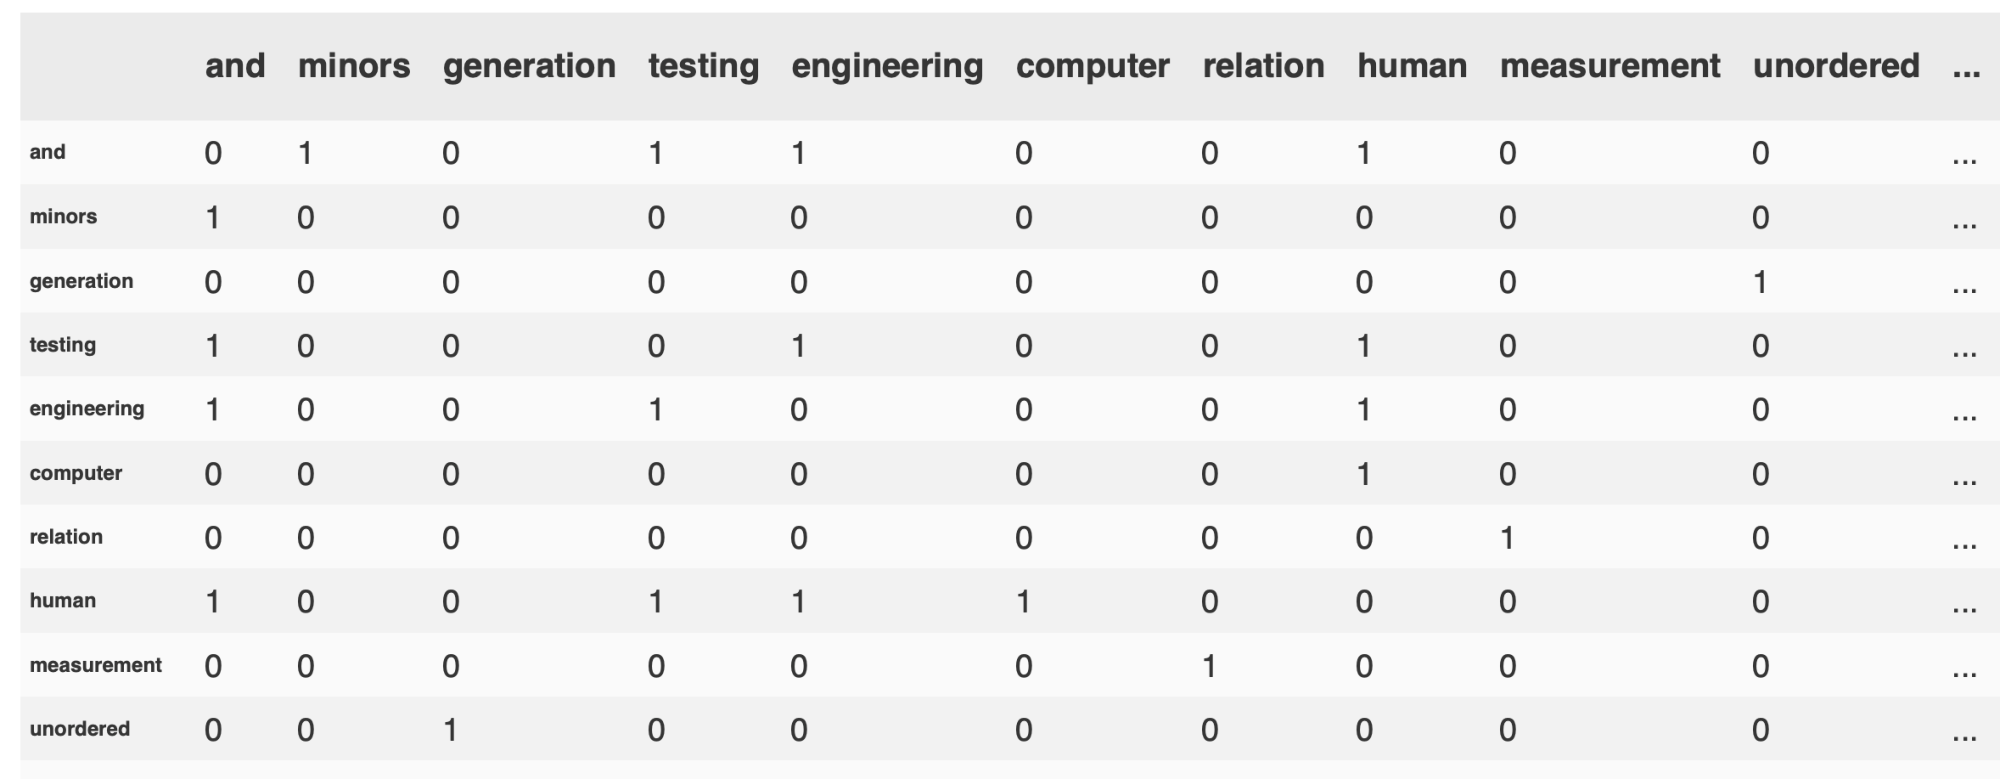
\includegraphics[scale=.4]{figures/wordvectors/wcm}	
\end{center}
\end{frame}

\begin{frame}
\frametitle{Singular Value Decomposition}
\begin{itemize}[<+->]
\item Collect $X = |V| \times |V|$ word co-occurrence matrix.
\item Apply SVD on $X$ to get $X = U S V^T$
\pause
\begin{block}{Transpose}
Transpose of $V$ is $V^T$ which switches the row and column of $V$
\end{block}
\item Select first $k$ columns of $U$ to get $k$-dimensional vectors
\item The matrix $S$ is a diagonal matrix with entries $\sigma_1, \ldots, \sigma_i, \ldots, \sigma_{|V|}$
\end{itemize}
\pause 
\begin{alertblock}{Variance}
The amount of variance captured by the first $k$ dimensions is given by
\[ \frac{\sum_{i=1}^k \sigma_i}{\sum_{i=1}^{|V|} \sigma_i} \]\end{alertblock}
\end{frame}

\begin{frame}
\frametitle{Dimensionality reduction with SVD}
\framesubtitle{Figure from \cite{cs224n}}
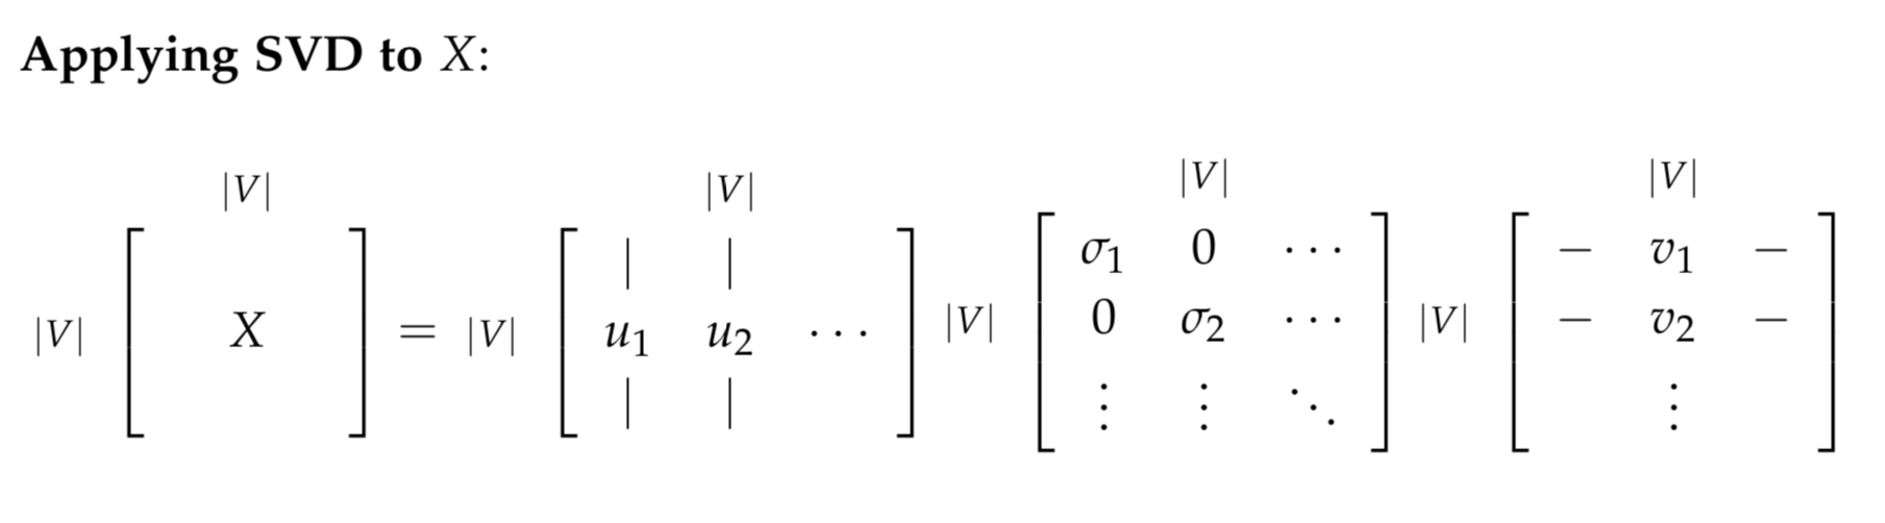
\includegraphics[scale=.38]{figures/wordvectors/svdapply}	
\end{frame}

\begin{frame}
\frametitle{Dimensionality reduction with SVD}
\framesubtitle{Figure from \cite{cs224n}}
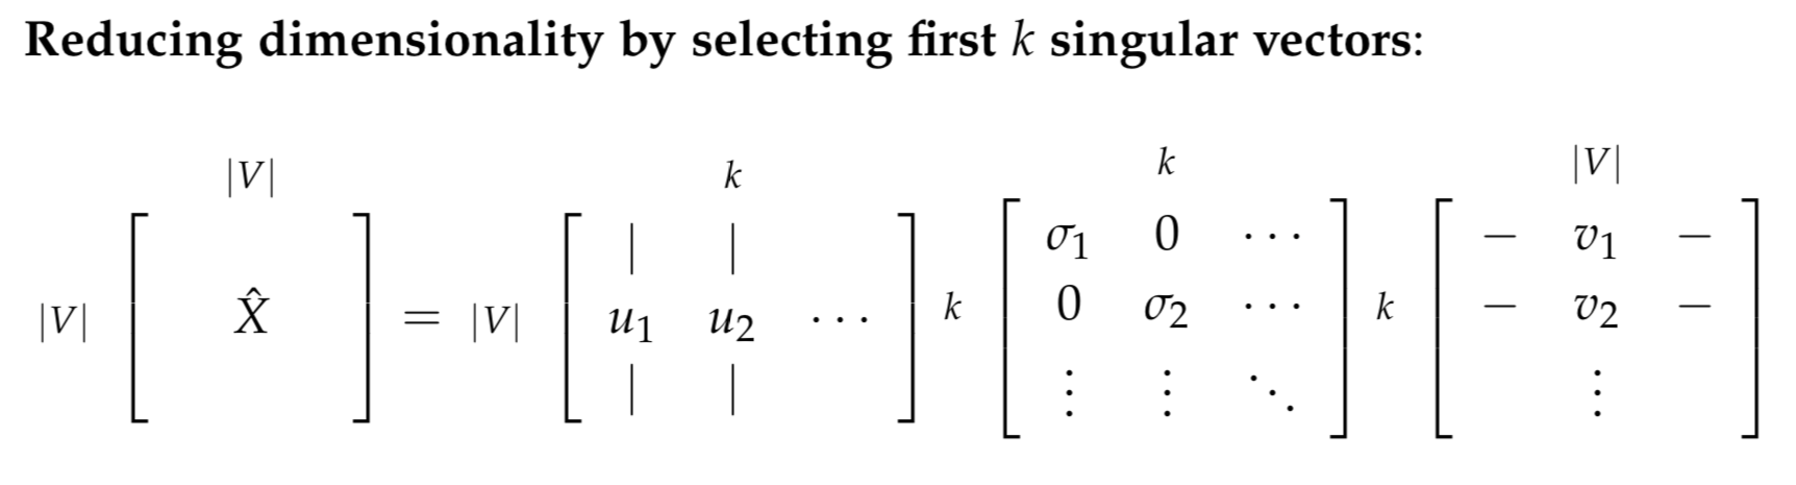
\includegraphics[scale=.38]{figures/wordvectors/reducedim}	
\end{frame}

\begin{frame}
\frametitle{Why SVD is not the ideal solution}
\begin{itemize}[<+->]
	\item Computational complexity is high ${\cal O}(|V|^3)$
	\item Cannot be trained as part of a larger model. 
	\item It is not a component that can be part of a larger neural network
	\item Cannot be trained discriminatively for a particular task
\end{itemize}
\end{frame}

\section{Word2Vec}
\frame{\tableofcontents[currentsection]}

\begin{frame}
\frametitle{Word2Vec}
\begin{itemize}[<+->]
	\item Word2Vec is a family of model + learning algorithm
	\item The goal is to learn dense word vectors
\end{itemize}
\pause
\begin{alertblock}{Continuous bag of words}
	\begin{itemize}[<+->]
		\item Takes the average of the context; predicts the target word
		\item Trained with gradient descent on cross entropy loss for word prediction 
	\end{itemize}
\end{alertblock}
\pause
\begin{alertblock}{Skip-gram}
	\begin{itemize}[<+->]
		\item Considers each context word independently and constructs (target-word, context-word) pairs
		\item Trained trained using negative sampling and loss on predicting good vs.\ bad pairs
	\end{itemize}
\end{alertblock}
\end{frame}

\begin{frame}
\frametitle{Word2Vec: Continuous Bag of Words}
\begin{alertblock}{CBOW}
\begin{tabbing}
the \= general \= commanded \= the \= troops\kill \\
the \> general \> \rlap{\underline{\hphantom{commanded}}} \> the \> troops
\end{tabbing}
Predicting a center word from the surrounding words \\
(also window-based)
\end{alertblock}
\pause 
\begin{block}{For each word we want to learn two vectors:}
\begin{itemize}
	\item $v_i \in \mathbb{R}^k$ (input vector) when the word $w_i$ is in the context
	\item $u_i \in \mathbb{R}^k$ (output vector) when the word $u_i$ is in the center 
\end{itemize}
\end{block}
\end{frame}

\begin{frame}
\frametitle{Word2Vec: Continuous Bag of Words}
\begin{block}{Algorithm}
\begin{tabbing}
the \= general \= commanded \= the \= troops\kill \\
the \> general \> \rlap{\underline{\hphantom{commanded}}} \> the \> troops \\
$v_{\textrm{the}}$ \> $v_{\textrm{general}}$ \> \> $v_{\textrm{the}}$ \> $v_{\textrm{troops}}$ 
\end{tabbing}
\begin{itemize}[<+->]
	\item Average the context vectors:
	\[ \hat{v} = \frac{v_{\textrm{the}} + v_{\textrm{general}} + v_{\textrm{the}} + v_{\textrm{troops}}}{4} \]
	\item For each word $i \in V$ we have a word vector $u_i \in \mathbb{R}^k$
	\item Compute the dot product $z_i = u_i \cdot \hat{v}$
	\item Convert $z_i \in \mathbb{R}$ into a probability:
	\[ \hat{y}_i = \frac{exp(z_i)}{\sum_{k=1}^{|V|} exp(z_k)} \]
	\item If the correct center word is $w_i$ then the max should be $\hat{y}_i$.
\end{itemize}	
\end{block}
\end{frame}

\begin{frame}
\frametitle{Word2Vec: Continuous Bag of Words}
\begin{tabbing}
the \= general \= commanded \= the \= troops\kill \\
the \> general \> \rlap{\underline{\hphantom{commanded}}} \> the \> troops \\
$v_{\textrm{the}}$ \> $v_{\textrm{general}}$ \> \> $v_{\textrm{the}}$ \> $v_{\textrm{troops}}$ 
\end{tabbing}
\begin{itemize}[<+->]
	\item Average the context vectors to get $\hat{v}$
	\item Let matrix $U = [ u_1, \ldots, u_{|V|} ] \in \mathbb{R}^{|V| \times k}$ with word vectors $u_i \in \mathbb{R}^k$
	\item Compute the matrix product $z = U \cdot \hat{v}$ where $z = [ z_1, \ldots, z_{|V|} ] \in \mathbb{R}^{|V|}$ and each $z_i \in \mathbb{R}$
	\item Compute vector $\hat{y} \in \mathbb{R}^{|V|}$. Each element $\hat{y}_i = \frac{exp(z_i)}{\sum_{k=1}^{|V|} exp(z_k)} $
	\item We write this as $\hat{y} = \textrm{softmax}(z)$
	\item If the correct center word is $w_i$ then the ideal output $y$ is a one-hot vector with index $i$ as 1 and all other elements are 0.
\end{itemize}
\end{frame}

\begin{frame}
\frametitle{Word2Vec: Continuous Bag of Words}
\begin{block}{Learning}
\begin{itemize}[<+->]
	\item Goal: learn $k$-dimensional word vectors $u_i, v_i$ for each $i = 1, \ldots |V|$
	\item For each training example the correct center word $w_j$ is represented as a one-hot vector $y$ where $y_j = 1$.
	\item $\hat{y} = \textrm{softmax}(U \cdot \hat{v})$ where $\hat{v}$ is the average of the context words
	\item Loss function is the cross entropy:
	\[ H(\hat{y}, y) = - \log(\hat{y}_j) \textrm{ for $j$ where $y_j = 1$} \]
	\item If $c$ is the index of the correct word, consider case where prediction $\hat{y}_c = 0.99$ then the loss or penalty is low $H(\hat{y}, y) = 1 \cdot \log(0.99) = 0.01$
	\item If the prediction was bad $\hat{y}_c = 0.01$ then the loss is high $H(\hat{y}, y) = 1 \cdot \log(0.01) = 4.6$
\end{itemize}	
\end{block}
\end{frame}

\begin{frame}
\frametitle{CBOW Loss Function}
\framesubtitle{Figure from \cite{melamud16}}
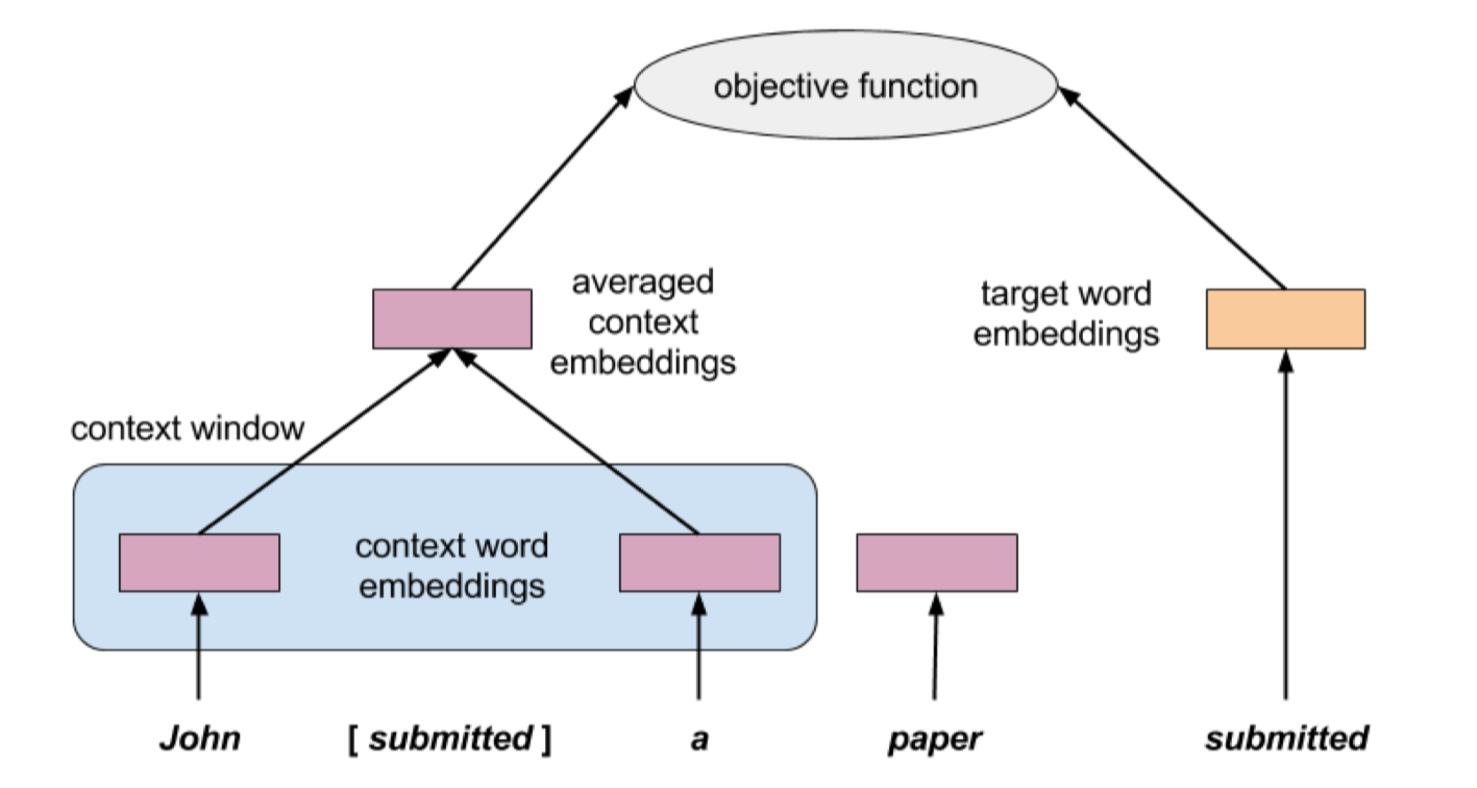
\includegraphics[scale=.45]{figures/wordvectors/cbowloss}	
\end{frame}

\begin{frame}
\frametitle{Gradient descent}
\begin{block}{Objective function}
\begin{eqnarray*}
\lefteqn{\textrm{Minimize } J } \\
& = & - \log P(u_c \mid \hat{v}) \\
& = & - u_c \cdot \hat{v} + \log \sum_{j=1}^{|V|} exp(u_j \cdot \hat{v})
\end{eqnarray*}
\end{block}
\end{frame}


\begin{frame}
\frametitle{Gradient descent}
\begin{itemize}[<+->]
\item Initialize $u^{(0)}$ and $v^{(0)}$ 
\item $J(u,v) = - u_c \cdot \hat{v} + \log \sum_{j=1}^{|V|} exp(u_j \cdot \hat{v})$
\item $t \leftarrow 0$
\item Iterate to minimize loss $H(\hat{y}, y)$ on each training example:
\begin{itemize}[<+->]
\item Pick a training example at random
\item Calculate: 
\begin{eqnarray*}
	\hat{y} &=& \textrm{softmax}(U \cdot \hat{v}) \\
	\Delta_u &=& \left. \frac{d J(u,v)}{d u}  \right|_{u,v = u^{(t)}, v^{(t)}} \\
	\Delta_v &=& \left. \frac{d J(u,v)}{d v}  \right|_{u,v = u^{(t)}, v^{(t)}}
\end{eqnarray*}
\item Using a learning rate $\gamma$ find new parameter values:
\begin{eqnarray*}
	\textbf{u}^{(t+1)} &\leftarrow& \textbf{u}^{(t)} - \gamma \Delta_u \\
	\textbf{v}^{(t+1)} &\leftarrow& \textbf{v}^{(t)} - \gamma \Delta_v
\end{eqnarray*}
\end{itemize}
\end{itemize}
\end{frame}

\section{GloVe}
\frame{\tableofcontents[currentsection]}

\begin{frame}
\frametitle{GloVe}
\begin{alertblock}{Co-occurrence matrix}
Let $X$ denote the word-word co-occurrence matrix.\\
$X_{ij}$ is number of times word $j$ occurs in the context of word $i$.\\
Let $X_i = \sum_k X_{ik}$ \\
And $P_{ij} = P(w_j \mid w_i) = \frac{X_{ij}}{X_i}$	
\end{alertblock}
\pause
\begin{alertblock}{Least-squares objective}
Probability that word $j$ occurs in context of word $i$:
\[ Q_{ij} = \frac{exp(u_j \cdot v_i)}{\sum_{w=1}^{|V|} exp(u_w \cdot v_i) } \]
Compute global cross-entropy loss:
\[ J = - \sum_{i=1}^{|V|} \sum_{j=1}^{|V|} X_{ij} \log Q_{ij} \]
\end{alertblock}
\end{frame}

\begin{frame}
\frametitle{GloVe}
\begin{alertblock}{Simplify objective function}
\[ J = - \sum_{i=1}^{|V|} \sum_{j=1}^{|V|} X_{ij} \log Q_{ij} \]
The distribution $Q_{ij}$ requires an expensive normalization over the entire vocabulary.
So we simplify $J$ to $\hat{J}$:
\[ \hat{J} = - \sum_{i=1}^{|V|} \sum_{j=1}^{|V|} X_i ( X_{ij} - \exp(u_j \cdot v_i) )^2 \]
The GloVe model efficiently leverages global statistical information by training only on the nonzero elements in a word-word co-occurrence matrix.
\end{alertblock}
\end{frame}


\begin{frame}
\setbeamertemplate{bibliography item}[text]
\begin{thebibliography}{10}

\bibitem{cs224n}
\alert{Christopher Manning, Richard Socher, Francois Chaubard, Michael Fang, Guillaume Genthial, Rohit Mundra.}
\newblock {Natural Language Processing with Deep Learning: Word Vectors I: Introduction, SVD and Word2Vec}
\newblock Winter 2019.


\bibitem{melamud16}
\alert{O. Melamud and J. Goldberger and I. Dagan}
\newblock context2vec: Learning Generic Context Embedding with Bidirectional LSTM.
\newblock CoNLL 2016.
\end{thebibliography}
\end{frame}


\section*{Acknowledgements}

\begin{frame}
\centering
\begin{alertblock}{Acknowledgements}
Many slides borrowed or inspired from lecture notes by Michael Collins, Chris Dyer, Kevin Knight, Philipp Koehn, Adam Lopez, Graham Neubig and Luke Zettlemoyer from their NLP course materials. 

\bigskip

All mistakes are my own.

\bigskip

A big thank you to all the students who read through these notes and helped me improve them.

\end{alertblock}
\end{frame}



\end{document}

